
\chapter{An Overview of High-Speed Link Systems}
\graphicspath{{An Overview of High-Speed Link Systems/Vector/}{An Overview of High-Speed Link Systems/}}

A typical high-speed link system consists of 3 basic components: a 
serializing transmitter, a communication channel, and a deserializing receiver, as 
shown on the block diagram in Figure 2.1.

\begin{figure*}
	\centering
	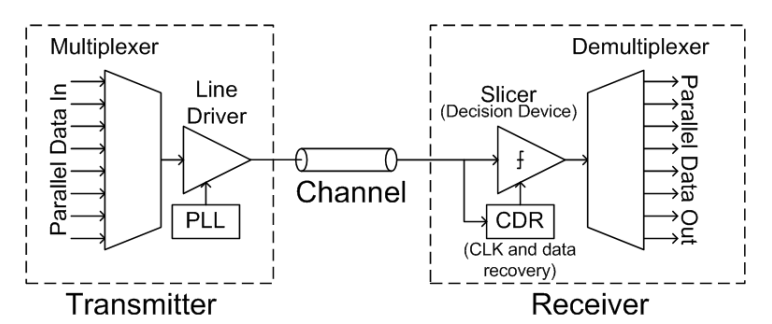
\includegraphics[width=14cm,height=6cm]{fig2_1.png}
	\caption{Block diagram of a high-speed link [5]}
	\label{high_sp_bl_diag}
\end{figure*}

The transmitter usually includes a multiplexer that converts parallel 
data into serial stream, a line driver that send data bits through the physical channel, 
and a clock source, usually implemented as a phase-locked loop (PLL). \\
The receiver decides which discrete digital value has most likely been 
transmitted. The decision device is usually referred to as slicer or comparator. Then 
the serial data stream is usually demultiplexed into parallel word, more naturally 
suited for data processing. If no explicit clock signal is sent along with the data, a clock and data recovery (CDR) block is needed to derive the timing information 
from data transitions.\\

A convenient way of describing a channel is by the pulse response of the channel. A pulse response of the channel is its output resulting from 
an isolated single-bit pulse (…0001000…) at its input. A general low-pass nature of 
most channels suggests that they cannot instantaneously respond to infinitely sharp 
edges of a pulse, delaying and dispersing it, as shown in Figure 2.2. When such pulse 
response is sampled at bit times, the largest sample is called the cursor; the samples 
before the cursor are called pre-cursors, and the samples after the cursors are called post-cursors. Pre-cursors interfere with previously sent bits, while post-cursors 
interfere with the following bits. To cancel such inter-symbol interference, most 
modern links use equalization. An equalizer provides an inverse channel response 
such that the overall frequency response is flat over the bandwidth of interest.

\begin{figure*}[h]
	\centering
	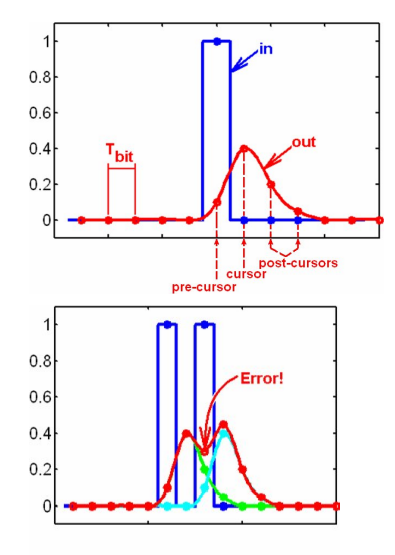
\includegraphics[width=6cm,height=10cm]{fig2_2.png}
	\caption{Pulse dispersion and inter-symbol interference [5]}
	\label{ISI}
\end{figure*}

%%%%%%%%%%%%%%%%%
%%%%%%%%%%%%%%%%%%
%%%%%% Chapter 2 Section 1
%%%%%%%%%%%%%%%%%
%%%%%%%%%%%%%%%%%%
\section{Linear Equalization}
Equalization is an important application space for digital-to-analog and 
analog-to-digital converters. Equalizer implementations fall into 3 general categories: 
analog, semi-digital, and digital. As we shall see, this classification is somewhat 
oversimplified, because most "analog" equalizers incorporate some digital adjustment, 
while all "digital" equalizers require ADCs and DACs to interface digital processors with analog channels. In fact, most equalizers operate on both analog and digital 
signals, so ADCs and DACs are needed to perform the conversion between the two 
domains. It is mainly equalizers that drive the development of data converters in high-speed links. To understand how ADCs can be optimized for this purpose, let us 
describe a few most common equalization techniques used in high-speed links.

\section{Digital Feedback Equalization}
\rhead{Digital Feedback Equalization}

All linear equalizers suffer from another problem. Ideally, an equalizer 
placed at the transmitter would boost a signal at high frequencies leaving low-frequency content intact. However, due to limited voltage swing of the channel driver, 
the filter is forced to attenuate lower frequencies rather than amplify higher 
frequencies, reducing the total signal energy and, thus, the signal-to-noise ratio (SNR). 
On the other hand, an equalizer placed at the receiver amplifies high-frequency noise 
along with the signal, again degrading the SNR.\\

To circumvent such noise amplification problem, non-linear equalizers 
can be used. The simplest, efficient, and thus most common non-linear equalizer used 
in high-speed link receivers is a decision-feedback equalizer (DFE), depicted in 
Figure 2.3 for a 4-tap example. Assuming that the 4 previous bits were detected 
correctly, DFE subtracts their influence from the currently received analog input 
voltage, thus cancelling their post-cursor ISI. Note that DFE cannot cancel pre-cursor 
ISI, because the cursor bit has not been sliced yet.

\begin{figure*}[h]
	\centering
	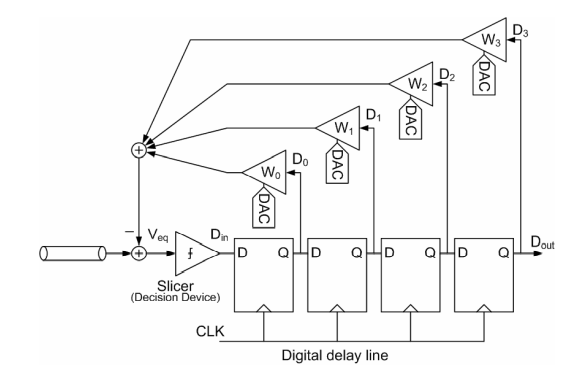
\includegraphics[width=12cm,height=8cm]{fig2_3.png}
	\caption{Decision-feedback equalizer on the receiver side
[5]}
	\label{DFE}
\end{figure*}

Nevertheless, DFE is very useful, because due to its non-linear nature 
(it contains a comparator), it does not amplify high-frequency noise from the channel. 
It is susceptible to error propagation, however, meaning that if a bit has been 
incorrectly detected, its ISI will not be corrected properly, leading to error propagating 
to the current bit. While this may cause chains of errors in low-SNR channels (like 
wireless), such error propagation is much less probable in higher-reliability short-reach copper links.


\section{Digital Equalizer Implementations}
\rhead{Digital Equalizer Implementations}

Implementing a filter in digital domain allows one to compute filtering 
results with higher resolution in digital domain and then round them off only once to 
the closest data converter level. This is in contrast with semi-digital implementation, 
where the value of each tap is rounded off, leading to accumulation of rounding errors. 
This problem is illustrated in Figure 2.4. Only three taps are shown for simplicity, but 
one can imagine the problem only getting worse for more taps. 
To understand this issue more fully, we can view the operation of the 
filter as a function of data bits as moving along a tree. The "root" of the tree is output 
for no filter taps. For one single tap, depending whether the previous data bit was 0 or 
1, the filter output branches to either (–W0) or W0. If the filter has two taps, depending 
on whether data bits were 00, 01, 10, or 11, there are four possibilities for the filter 
output: (-W1,-W0), (-W1,+W0), (+W1,-W0), and (+W1,+W0). For 3 taps, there are 8 possible 
outputs, and for $N_{taps} \  taps \,–\,
2^{N_{taps}}$ . Figure 2.4(a) shows the tree without any 
quantization. Figure 2.4(b) illustrates how quantization of each individual tap weight 
leads to error accumulation. Finally, Figure 2.4(c) shows that computing filter output 
with higher precision in digital domain and then rounding solves the error 
accumulation problem.\\

\begin{figure*}[h]
	\centering
	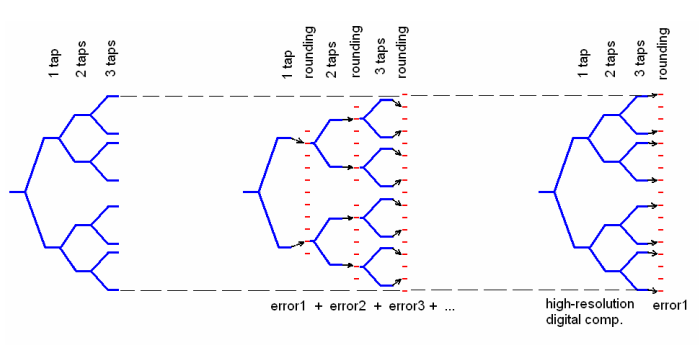
\includegraphics[width=12cm,height=8cm]{fig2_4.png}
	\caption{FIR filter output as a function of input bits (a) without any quantization, (b) 
with each tap weight Wi quantized separately, and (c) with filter output computed 
digitally with high resolution and then rounded off to the closest available data 
converter level [5]}
	\label{dig_fil_err_acc}
\end{figure*}

Unfortunately, implementing a digital filter at high speed and with high 
resolution is also problematic. Thus, instead of performing digital computations on-the-fly, look-up tables (LUTs) can be used, as demonstrated by B. Casper, et. al. in 
[6] for transmit equalization.



\section{ADC for Receiver Equalization}
\rhead{ADC for Receiver Equalization}

Apart from digital filters, the digital transmit equalizer requires a baud-rate 
DAC, while the digital receive equalizer requires a baud-rate ADC. As baud rates of 
modern links extend well into Gbps range, both DACs and ADCs operating at such 
rates are large research topics in themselves. In this work, we focus only on designing 
high-speed ADCs for the link receivers. The complexity, and even feasibility, of this 
task as well as the choice of the ADC topology depend on system requirements for the 
ADC. While the baud rate of the link determines the sampling rate of the ADC, its 
resolution is defined by two considerations. \\
First, the LSB size must be small enough so that it does not noticeably degrade 
the noise margin of the link, defined by half a signal swing minus all bounded error 
sources. Equalization normally removes the precursor and postcursor ISI, leaving only 
the main cursor as a signal to be detected and reducing the useful signal swing by the 
sum of magnitudes of all pre- and post-cursors. On top of this attenuation, the bounded 
error sources include unequalized ISI, reflections, and crosstalk. The ADC 
quantization error becomes an additional bounded error source, and thus should be 
kept to a small fraction $\alpha$ of the main cursor. The value of $\alpha$ should be typically less 
than 10-20%. 
\\
Second, the ADC range must cover the entire swing of the receiver input, 
including the worst-case effects from the pre- and post-cursor ISI (unless they have 
been cancelled by the transmit equalizer). The worst-case signal swing is equal to the 
sum of magnitudes of all taps in a pulse response (pre- and post-cursors plus the cursor 
itself).\\
Given these two considerations, the number of ADC levels ( $$ N_{levels}=2^{N_{bits}} $$ ) 
should be approximately: 

$$ N_{levels}=2^{N_{bits}}=\sum_{i=-\infty}^{\infty} |P_i|/{\alpha.P_0} $$\\

where $P_{i}$ is the $i{th}$ tap in a channel pulse response, with i < 0 for pre-cursors, i > 0 for post-cursors and i = 0 for the main-cursor. $\alpha$ is the fraction of equalized signal 
amplitude allocated to quantization error of the ADC. Taking $\alpha$ = 10\% and pulse 
response shown in Figure 2.2 as an example, we obtain $N{levels} = 20 \ and\  N{bits} = 4.3$. As it 
turns out, for most typical backplane channels, N{bits} of 4-5 bits is required. Thus, for 
this work, we will target a resolution of 6-7 bits.


